Before we can define variability parity games we first define \textit{featured parity games} (FPG), featured parity games extend the definition of parity games to capture the variability represented in an FTS. It uses the same concepts as FTSs: features, products and a function that guards edges. In this section we will introduce the definition of FPGs and show that solving them answers the verification questions for FTS: For which products in the FTS does its projection satisfy $\varphi$?

First we introduce the definition of an FPG:
\begin{definition}
	\label{def_FPG}
	A featured parity game (FPG) is a tuple $(V,V_0, V_1, E, \Omega, N, P, \gamma)$, where:
	\begin{itemize}
		\item $V = V_0 \cup V_1$ and $V_0 \cap V_1 = \emptyset$,
		\item $V_0$ is the set of vertices owned by player $0$,
		\item $V_1$ is the set of vertices owned by player $1$, 
		\item $E \subseteq V \times V$ is the edge relation,
		\item $\Omega :  V \rightarrow \mathbb{N}$ is a priority assignment,
		\item $N$ is a non-empty set of features,
		\item $P \subseteq \mathcal{P}(N)$ is a non-empty set of products, ie. feature assignments, for which the game can be played,
		\item $\gamma : E \rightarrow \mathbb{B}(N)$ is a total function, labelling each edge with a Boolean expression over the features.
	\end{itemize}
\end{definition}
An FPG is played similarly to a PG, however the game is played for a specific product $p \in P$. Player $\alpha$ can only move the token from $v \in V_\alpha$ to $w \in V$ if $(v,w) \in E$ and $p \models \gamma(v,w)$.

A game played for product $p \in P$ results in winnings sets $W_0^p$ and $W_1^p$, which are defined similar to the $W_0$ and $W_1$ winning sets for parity games.

An FPG can simply be projected to a product $p$ by removing the edges that are not satisfied by $p$.
\begin{definition}
	\label{def_FPG_proj}
The projection from FPG $G = (V,V_0, V_1, E, \Omega, N, P, \gamma)$ to a product $p \in P$, noted $G_{|p}$, is the parity game $(V,V_0,V_1, E', \Omega)$ where $E' = \{ e \in E\ |\ p \models \gamma(e) \}$.
\end{definition}

Playing FPG $G$ for a specific product $p\in P$ is the same as playing the PG $G_{|p}$. Any path that is valid in $G$ for $p$ is also valid in $G_{|p}$ and vice versa. Therefore the strategies are also interchangeable, furthermore the winning sets $W_\alpha$ for $G_{|p}$ and $W_\alpha^p$ for $G$ are identical. Since parity games are positionally determined so are FPGs. Similarly, since finite parity games are decidable, so are finite FPGs.

We say that an FPG is solved when the winning sets for every valid product in the FPG are determined.
\subsection{Creating featured parity games}
An FPG can be created from an FTS in combination with a model $\mu$-calculus formula. We translate an FTS to an FPG by first creating a PG from the transition system as if there were no transition guards, next we apply the same guards to the FPG as are present in the FTS for edges that originate from transitions. The features and valid products in the FPG are identical to those in the FTS.
\begin{definition}
	\label{def_FTS2FPG}
	$FTS2FPG(M, \varphi)$ converts FTS $M = (S, Act, trans, s_0, N, P, \gamma)$ and closed formula $\varphi$ to FPG $(V, V_0, V_1, E, \Omega, N, P, \gamma')$.
	
	We have $(V, V_0, V_1, E, \Omega) = \textit{LTS2PG}((S, Act, trans, s_0), \varphi$) and
	\[ \gamma'((s, \psi),(s', \psi')) = \begin{cases}
	\gamma(s,a,s') & \text{if }\psi = \langle a \rangle \psi'\text{ or }\psi = [a]\psi' \\
	\top & \text{otherwise}
	\end{cases}\]
\end{definition}
Consider our working example which we extend to an FTS depicted in figure \ref{fig:exverfts}, for this example we have features $N = \{f, g\}$ and products $P = \{\emptyset, \{f\},\{f,g\}\}$.
\begin{figure}[h]
	\centering
	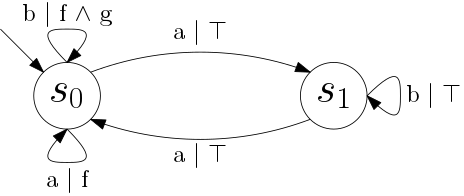
\includegraphics[scale=0.3]{Examples/ExamleVerification/FTS}
	\caption[FTS $M$]{FTS $M$}
	\label{fig:exverfts}
\end{figure}
\begin{figure}[h]
	\centering
	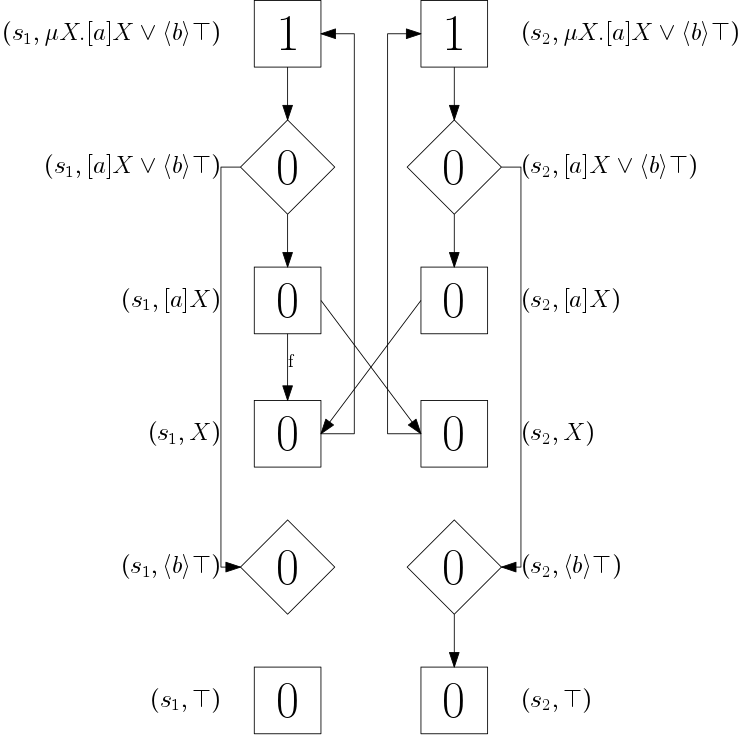
\includegraphics[scale=0.3]{Examples/ExamleVerification/FPG}
	\caption[FPG for $M$ and $\varphi$]{FPG for $M$ and $\varphi$}
	\label{fig:exverfpg}
\end{figure}
We can translate this FTS with formula $\varphi = \mu X. ([a] X \vee \langle b \rangle \top)$ to an FPG depicted in figure \ref{fig:exverfpg}. As we can see from the FTS if feature $f$ is enabled and $g$ is disabled then we have an infinite path of $a$'s where $b$ is never enabled, therefore $\varphi$ doesn't hold for $M_{|\{f\}}$. If $g$ is enabled however we can always do a $b$ so $\varphi$ holds for $M_{|\{f,g\}}$. As we have seen $\varphi$ does hold for $M_{|\emptyset}$. For the product $\emptyset$ we have the same winning set as before:
\begin{align*}
W_0^\emptyset = \{& (s_1, \mu X.[a]X \vee \langle b \rangle \top),\\
& (s_1, [a]X \vee \langle b \rangle \top),\\
& (s_1, [a]X),\\
& (s_1, X),\\
& (s_1, \top),\\
& (s_2, \mu X.[a]X \vee \langle b \rangle \top),\\
& (s_2, [a]X \vee \langle b \rangle \top),\\
& (s_2, [a]X),\\
& (s_2, X),\\
& (s_2, \langle b \rangle \top),\\
& (s_2, \top)
\}\\
W_1^\emptyset = \{& (s_1, \langle b \rangle \top )\}
\end{align*}
In the FPG we can see that if $f$ is enabled and $g$ is disabled then player $1$ can move the token from $(s_1, [a]X)$ to $(s_1,X)$. This results in player $0$ either moving the token to $(s_1, \langle b \rangle \top)$ and losing or an infinite path where $1$ occurs infinitely often which is also player $1$ wins. For product $\{f\}$ we have winning sets:
\begin{align*}
W_0^{\{f\}} = \{
& (s_1, \top),\\
& (s_2, \mu X.[a]X \vee \langle b \rangle \top),\\
& (s_2, [a]X \vee \langle b \rangle \top),\\
& (s_2, X),\\
& (s_2, \langle b \rangle \top),\\
& (s_2, \top)
\}\\
W_1^{\{f\}} = \{& (s_1, \mu X.[a]X \vee \langle b \rangle \top),\\
& (s_1, [a]X \vee \langle b \rangle \top),\\
& (s_1, [a]X),\\
& (s_1, X),\\
& (s_1, \langle b \rangle \top ),\\
& (s_2, [a]X)\}
\end{align*}
However if $g$ is also enabled then player $0$ wins in $(s_1, \langle b \rangle \top)$, thus giving the following winning sets:
\begin{align*}
W_0^{\{f,g\}} = \{& (s_1, \mu X.[a]X \vee \langle b \rangle \top),\\
& (s_1, [a]X \vee \langle b \rangle \top),\\
& (s_1, [a]X),\\
& (s_1, X),\\
& (s_1, \langle b \rangle \top ),\\
& (s_1, \top),\\
& (s_2, \mu X.[a]X \vee \langle b \rangle \top),\\
& (s_2, [a]X \vee \langle b \rangle \top),\\
& (s_2, [a]X),\\
& (s_2, X),\\
& (s_2, \langle b \rangle \top),\\
& (s_2, \top)
\}\\
W_1^{\{f,g\}} = \{\}
\end{align*}

In the next section we will show how the winning sets relate to the model verification question.


\subsection{FTS verification using FPG}
We can create an FPG from an FTS and project it to a product, resulting in a PG, this is shown in the following diagram:\\
\begin{tikzpicture}
\matrix (m) [matrix of math nodes,row sep=4em,column sep=4em,minimum width=2em]
{
	\text{FTS} & \text{FPG} \\
	\  & \text{PG} \\};
\path[-stealth]
(m-1-1)
edge node [above] {$\varphi$} (m-1-2)

(m-1-2) edge [double] node [right] {$\Pi$} (m-2-2)
;
\end{tikzpicture}\\
Earlier we saw that we could also derive a PG by projecting the FTS to a product and then translation the resulting LTS to a PG, depicted by the following diagram:
\\\begin{tikzpicture}
\matrix (m) [matrix of math nodes,row sep=4em,column sep=4em,minimum width=2em]
{
	\text{FTS} \\
	\text{LTS} & \text{PG} \\};
\path[-stealth]
(m-1-1) edge [double] node [left] {$\Pi$} (m-2-1)
(m-2-1.east|-m-2-2) edge node [above] {$\varphi$}
(m-2-2)
;
\end{tikzpicture}\\
We will now show that the resulting parity games are identical.
\begin{theorem}
	\label{the_PGsubPGA} Given:
	\begin{itemize}
		\item FTS $M = (S,Act, trans, s_0, N, P, \gamma)$,
		\item a closed modal mu-calculus formula $\varphi$,
		\item a product $p \in P$
	\end{itemize}
	it holds that the parity games LTS2PG($M_{|p}, \varphi$) and FTS2FPG($M, \varphi$)$_{|p}$  are identical.
	\begin{proof}
		Let $G^F = (V^F, V_0^F, V_1^F, E^F, \Omega^F, N, P, \gamma') = FTS2FPG(M, \varphi)$, using definition \ref{def_FTS2FPG}, and $G^F_{|p} = (V^F, V_0^F, V_1^F, {E^F}', \Omega^F)$, using definition \ref{def_FPG_proj}. Furthermore we have $M_{|p} = (S, Act, trans', s_0)$ and we let $G = (V, V_0, V_1, E, \Omega) =  LTS2PG(M_{|p}, \varphi)$. We depict the different transition systems and games in the following diagram.
		
		\begin{tikzpicture}
		\matrix (m) [matrix of math nodes,row sep=4em,column sep=1em,minimum width=2em]
		{
			\text{\ \ FTS }M & \  &\ & \text{FPG } G^F  \\
			\text{LTS }M_{|p} & \ & \text{PG } G & \text{\ \ PG }G_{|p}^F \\};
		\path[-stealth]
		(m-1-1) edge [double] node [left] {$\Pi$} (m-2-1)
		edge node [above] {$\varphi$} (m-1-4)
		(m-2-1.east|-m-2-3) edge node [above] {$\varphi$}
		(m-2-3)
		(m-1-4) edge [double] node [right] {$\Pi$} (m-2-4);
		\end{tikzpicture}\\
		We will prove that $G = G_{|p}^F$. We first note that game $G$ is created by 
		\[  (V, V_0, V_1, E, \Omega) = LTS2PG((S, Act, trans', s_0),\varphi) \]
		and the vertices, edges and priorities of game $G^F$ are created by 
		\[ (V^F, V_0^F, V_1^F, E^F, \Omega^F) = LTS2PG((S,Act, trans, s_0), \varphi)\]
		Using the definition of LTS2PG (\ref{def_LTS2PG}) we find that the vertices and the priorities only depend on the states in $S$ and the formula $\varphi$, since these are identical in the above two statements we immediately get $V = V^F, V_0 = V_0^F, V_1 = V_1^F$ and $\Omega = \Omega^F$. The vertices and priorities don't change when an FTS is projected, therefore $G_{|p}^F$ has the same vertices and priorities as $G^F$.
		
		Now we are left with showing that $E = {E^F}'$ in order to conclude that that $G = G^F_{|p}$. We will do this by showing $E \subseteq {E^F}'$ and $E \supseteq {E^F}'$.
		
		First let $e \in E$. Note that a vertex in the parity game is represented by a pair of a state and a formula. So we can write $e = ((s,\psi),(s',\psi'))$. To show that $e \in {E^F}'$ we distinguish two cases:
		\begin{itemize}
			\item  If $\psi = \langle a \rangle \psi'$ or $\psi = [a] \psi'$ then there exists an $a \in Act$ such that $(s,a,s') \in trans'$. Using the FTS projection definition (\ref{def_fts_proj}) we get $(s,a,s') \in trans$ and $p \models \gamma(s,a,s')$. Using the FTS2FPG definition (\ref{def_FTS2FPG}) we find that $\gamma'((s,\psi),(s',\psi')) = \gamma(s,a,s')$ and therefore $p \models \gamma'((s,\psi),(s',\psi'))$. Now using the FPG projection definition (\ref{def_FPG_proj}) we find $((s,\psi),(s',\psi')) \in {E^F}'$.
			\item Otherwise the existence of the edge does not depend on the $trans$ parameter and therefore $((s,\psi),(s',\psi')) \in {E^F}'$ if $(s,\psi) \in V^F$, since $V^F = V$ we have $(s,\psi) \in V^F$.
		\end{itemize}
		We can conclude that $E \subseteq {E^F}'$, next we will show $E \supseteq {E^F}'$. Let $e = ((s,\psi),(s',\psi')) \in {E^F}'$. We distinguish two cases:
		\begin{itemize}
			\item If $\psi = \langle a \rangle \psi'$ or $\psi = [a] \psi'$ then there exists an $a \in Act$ such that $(s,a,s') \in trans$. Using the FPG projection definition (\ref{def_FPG_proj}) we get $p \models \gamma'(s,a,s')$. Using the FTS2FPG definition (\ref{def_FTS2FPG}) we get $p \models \gamma(s,a,s')$. Using the FTS projection definition (\ref{def_fts_proj}) we get $(s,a,s') \in trans'$ and therefore $((s,\psi),(s',\psi'))\in E$.
			\item Otherwise the existence of the edge does not depend on the $trans$ parameter and therefore $((s,\psi),(s',\psi')) \in E$ if $(s,\psi) \in V$, since $V^F = V$ we have $(s,\psi) \in V$.
		\end{itemize}
	\end{proof}
\end{theorem}

Having proven this we can visualize the relation between the different games and transition systems in the following diagram:
\\\begin{tikzpicture}
\matrix (m) [matrix of math nodes,row sep=4em,column sep=4em,minimum width=2em]
{
	\text{FTS} & \text{FPG} \\
	\text{LTS} & \text{PG} \\};
\path[-stealth]
(m-1-1) edge [double] node [left] {$\Pi$} (m-2-1)
edge node [above] {$\varphi$} (m-1-2)
(m-2-1.east|-m-2-2) edge node [above] {$\varphi$}
(m-2-2)
(m-1-2) edge [double] node [right] {$\Pi$} (m-2-2)
;
\end{tikzpicture}\\
Finally we prove that solving an FTS, ie. finding winning sets for all products, answers the verification question.
\begin{theorem}
	\label{the_FPG_ver_FTS}
	Given:
	\begin{itemize}
		\item FTS $M = (S, Act, trans, s_0, N, P, \gamma)$,
		\item closed modal mu-calculus formula $\varphi$,
		\item product $p \in P$ and
		\item state $s \in S$
	\end{itemize}
	it holds that $(M_{|p}, s) \models \varphi$ if and only if $(s, \varphi) \in W_0^p$ in $\textit{FTS2FPG}(M, \varphi$).
	\begin{proof}
		The winning set $W_\alpha^p$ is equal to winning set $W_\alpha$ in $\textit{FTS2FPG}(M, \varphi)_{|p}$, for any $\alpha \in \{0,1\}$, using the FPG definition (\ref{def_FPG}). Using theorem \ref{the_PGsubPGA} we find that the game $FTS2FPG(M, \varphi)_{|p}$ is equal to the game $LTS2PG(M_{|p}, \varphi)$, obviously their winning sets are also equal. Using the well studied relation between parity games and LTS verification, stated in theorem \ref{the_LTS_PG_REL}, we know that $(M_{|p}, s) \models \varphi$ if and only if $(s, \varphi) \in W_0$ in game $LTS2PG(M_{|p},\varphi)$. Winning set $W_\alpha^p$ is equal to $W_\alpha$, therefore the theorem holds.
	\end{proof}
\end{theorem}

Revisiting our prior example we can see the theorem in action by noting that $M_{|\emptyset} \models \varphi$ , $M_{|\{f\}} \not\models \varphi$ and $M_{|\{f,g\}} \models \varphi$. This is reflected by the vertex $(s_1, \mu X. [a]X \vee \langle b \rangle \top)$ being present in $W_0^\emptyset$ and $W_0^{\{f,g\}}$ but not in $W_0^{\{f\}}$.